\clearpage
\setcounter{page}{1}
\maketitlesupplementary
%\todo{More results, maybe video, two pages like videocutler, what is selected high medium low quality, visual examples. show more examples per line 90\% 70\% 50\% ... so people can see what quality selector does}

% \section{Rationale}
% \label{sec:rationale}
% % 
% Having the supplementary compiled together with the main paper means that:
% % 
% \begin{itemize}
% \item The supplementary can back-reference sections of the main paper, for example, we can refer to \cref{sec:intro};
% \item The main paper can forward reference sub-sections within the supplementary explicitly (e.g. referring to a particular experiment); 
% \item When submitted to arXiv, the supplementary will already included at the end of the paper.
% \end{itemize}
% % 
% To split the supplementary pages from the main paper, you can use \href{https://support.apple.com/en-ca/guide/preview/prvw11793/mac#:~:text=Delete%20a%20page%20from%20a,or%20choose%20Edit%20%3E%20Delete).}{Preview (on macOS)}, \href{https://www.adobe.com/acrobat/how-to/delete-pages-from-pdf.html#:~:text=Choose%20%E2%80%9CTools%E2%80%9D%20%3E%20%E2%80%9COrganize,or%20pages%20from%20the%20file.}{Adobe Acrobat} (on all OSs), as well as \href{https://superuser.com/questions/517986/is-it-possible-to-delete-some-pages-of-a-pdf-document}{command line tools}.


\section{Detailed methodology}
\label{detailed_method}

This section supplements what is not clearly stated in \cref{sec:multi_round_training}.
% \begin{figure*}[ht]
%     \centering
%     \includegraphics[width=1\linewidth]{figures/method_overall.png}
%     \caption{
%         Our framework has two stages. In stage 1, we train the video instance segmentation (VIS) model and quality predictor on synthetic videos. We use the synthetic videos and models in stage 1 to initialize the training dataset and models in stage 2. In stage 2, we train the VIS model on the training dataset and use it to infer unlabeled videos. Then we use the quality predictor to select good quality results from videos labeled by the VIS model. In the end, we use the good-quality labeled videos to update our training set, which can be used for the next iteration.
%     }
%     \label{fig:overall_}
% \end{figure*}

% \cref{fig:overall_} shows the overall structure of our framework. Our method employs a dual-stage architecture. In stage 1, we train both the video instance segmentation (VIS) model and the quality predictor on synthetic videos from VideoCutLER~\cite{videocutler}. These components are subsequently leveraged to initialize both the training dataset and models for stage 2. In stage 2, we optimize the VIS model through iterative training on the established training dataset, then deploy it for pseudo-label generation on unlabeled video content. Following this, our quality predictor filters the machine-labeled outputs to retain only good-quality predictions. Ultimately, we update the training dataset with these quality-assured, curated annotations, enabling progressive enhancement through subsequent training cycles.
% \subsection{Stage 1}

% \subsubsection{Video Instance Segmentation (VIS) Model}

% Following~\cite{videocutler}, we use the VideoMask2Former~\cite{videomask2former, mask2former} with ResNet-50~\cite{resnet} backbone as our video instance segmentation (VIS) model.



% \subsubsection{Quality Predictor}

% For the quality predictor, we use an architecture very similar to~\cite{maskscore}. As shown in \cref{fig:predictor}, we use the first-layer features of the pixel decoder and the predicted mask as input. Employing a simple architecture with four convolution layers and three fully-connected layers, we predict the IoU of the predicted mask and ground truth in the end.

% Our architecture processes individual frame features and single-object mask predictions per inference step, contrasting with the VIS model's variable-length temporal-instance mask sequences. Supervision is established through threshold-binarized (0.5) mask IoU between predictions and matched ground truths, optimized via $\ell_2$ regression loss.

% While maintaining architectural alignment with~\cite{maskscore}, our key modification preserves continuous mask probabilities as model input, contrasting with the original binarized implementation. This adaptation proves critical as binarized inputs fundamentally impair quality predictor functionality in our framework.

% \subsubsection{Synthetic Videos}

% VideoCutLER~\cite{videocutler} provides a high-quality pseudo-labeled synthetic video dataset that was built on the unlabeled images from ImageNet~\cite{imagenet}, which is very suitable to train our VIS model and quality predictor in stage 1. We also use the trained VideoMask2Former model~\cite{videomask2former} from VideoCutLER to initialize our VIS model in stage 1. Instead of freezing the VIS model and training the quality predictor only, we found that training them both can lead to higher IoU prediction accuracy. 

% \subsection{Stage 2}

% In stage 2, we implement a four-phase self-training paradigm:
% \begin{enumerate}
%     \item Iterative parameter optimization of the VIS model on curated training data,
%     \item Automated pseudo-annotation of unlabeled video sequences with spatiotemporal non-Maximum suppression (NMS),
%     \item Confidence-aware filtration via our quality predictor, and
%     \item Dynamic dataset augmentation through adaptive fusion of newly curated annotations.
% \end{enumerate}

% This stage can run for multiple iterations until we get the final results.

% \subsubsection{Optimizing VIS model on Training Dataset}

% The training dataset is initialized using the synthetic videos from VideoCutLER~\cite{videocutler}. Following each update to the training dataset, we execute model parameter restoration from the first-stage model weights, thereby establishing a stable knowledge preservation mechanism within our progressive learning framework.

\subsection{Automated pseudo-annotation with spatio-temporal NMS}

After the training of the VIS model, we use it to label the unlabeled videos. 
Let $\mathcal{D} = \{d_i\}^{N}_{i=1}$ denote the initial detection set per video, where each detection $d = (s_i, \{m_i^t\}^{T}_{t=1})$ contains:
\begin{itemize}
    \item $s_i \in [0,1]$: Confidence score
    \item $\{m_i^t\}^{T}_{t=1}$: Binary mask sequence across $T$ frames
\end{itemize}

We filter those detections that have confidence scores larger than or equal to 0.25:
\begin{equation}
    \mathcal{D}_{\text{filtered}} = \{ d_i \in \mathcal{D} \mid s_i \geq 0.25 \}
\end{equation}

However, the detection sets may contain duplicate detections. To solve this problem, we need to perform spatiotemporal non-maximum suppression. First, we sort the detections based on their confidence scores:
\begin{equation}
    \mathcal{D}_{\text{sorted}} = \{ d_{(k)} \}_{k=1}^{|\mathcal{D}_{\text{filtered}}|} \quad \text{s.t.} \quad \forall i < j: s_{(i)} \geq s_{(j)}
\end{equation}

Our method eliminates redundant detections through spatiotemporal overlap analysis: Any lower-confidence prediction is suppressed if exhibiting mask overlap (IoU $\geq$ 0.5) with higher-confidence detections in at least one video frame. Formally, let $\mathcal{D}_{\text{suppressed}} \subseteq \mathcal{D}_{\text{sorted}}$ represent the preserved detection set after suppression:

\begin{equation}
\begin{split}
d_{(k)} \in \mathcal{D}_{\text{suppressed}} \iff & \nexists d_{(p)} \in \mathcal{D}_{\text{suppressed}} \ \text{where} \ p < k \ \text{s.t.} \\
& \exists t \in [1,T] : \frac{\|m_{(k)}^t \cap m_{(p)}^t\|}{\|m_{(k)}^t \cup m_{(p)}^t\|} \geq 0.5 \\
& \underbrace{\hphantom{\exists t \in [1,T] : \frac{\|m_{(k)}^t \cap m_{(p)}^t\|}{\|m_{(k)}^t \cup m_{(p)}^t\|}}}_{\mathclap{\text{Frame-specific overlap condition}}}
\end{split}
\end{equation}
where $\| \cdot \|$ denotes pixel cardinality. This temporal-existential criterion suppresses duplicates appearing in any frame of the video sequence.

\subsection{Confidence-aware filtration via quality predictor}

Let $\mathcal{D}_{\text{global}}^{(k)}$ denote the union of $\mathcal{D}_{\text{suppressed}}$ of all videos:
\begin{equation}
    \mathcal{D}_{\text{global}}^{(k)} = \bigcup_{v \in \mathcal{V}} \mathcal{D}_{\text{suppressed},v}^{(k)}
\end{equation}
where $\mathcal{D}_{\text{suppressed},v}^{(k)}$ denotes preserved detections for video $v$ after spatiotemporal NMS at iteration $k$.

For each detection $d \in \mathcal{D}_{\text{global}}^{(k)}$, we define:
\begin{equation}
    Q_d^t = s_d \cdot \hat{\text{IoU}}_d^t \quad \forall t \in [1,T_v]
\end{equation}
where $Q_d^t$ is the quality score of detection $d$ in frame $t$, $s_d$ is the confidence score of detection $d$, and $T_v$ denotes the number of frames in video $v$.

We implement quality-based pseudo-label selection using a fixed quality threshold $\tau_{\text{th}}$. For each detection $d \in \mathcal{D}_{\text{global}}^{(k)}$ across all videos:

\begin{equation}
    \mathcal{S}_d^t = \begin{cases} 
1 & Q_d^t \geq \tau^{(k)} \\
0 & \text{otherwise}
\end{cases}
\end{equation}
where $\mathcal{S}_d^t$ denote whether pseudo-label of detection $d$ in frame $t$ is selected. For each detection, if its results are not selected in any frames, we discard it:

\begin{equation}
\mathcal{D}_{\text{retained}}^{(k)} = \left\{ d_v \in \mathcal{D}_{\text{global}}^{(k)} \,\bigg|\, \sum_{t=1}^{T_v} \mathcal{S}_d^t > 0 \right\}
\end{equation}
where $\mathcal{D}_{\text{retained}}^{(k)}$ is the set of detections we retain in iteration $k$.



\section{Additional qualitative visualizations}

\begin{figure*}[h]
    \centering
    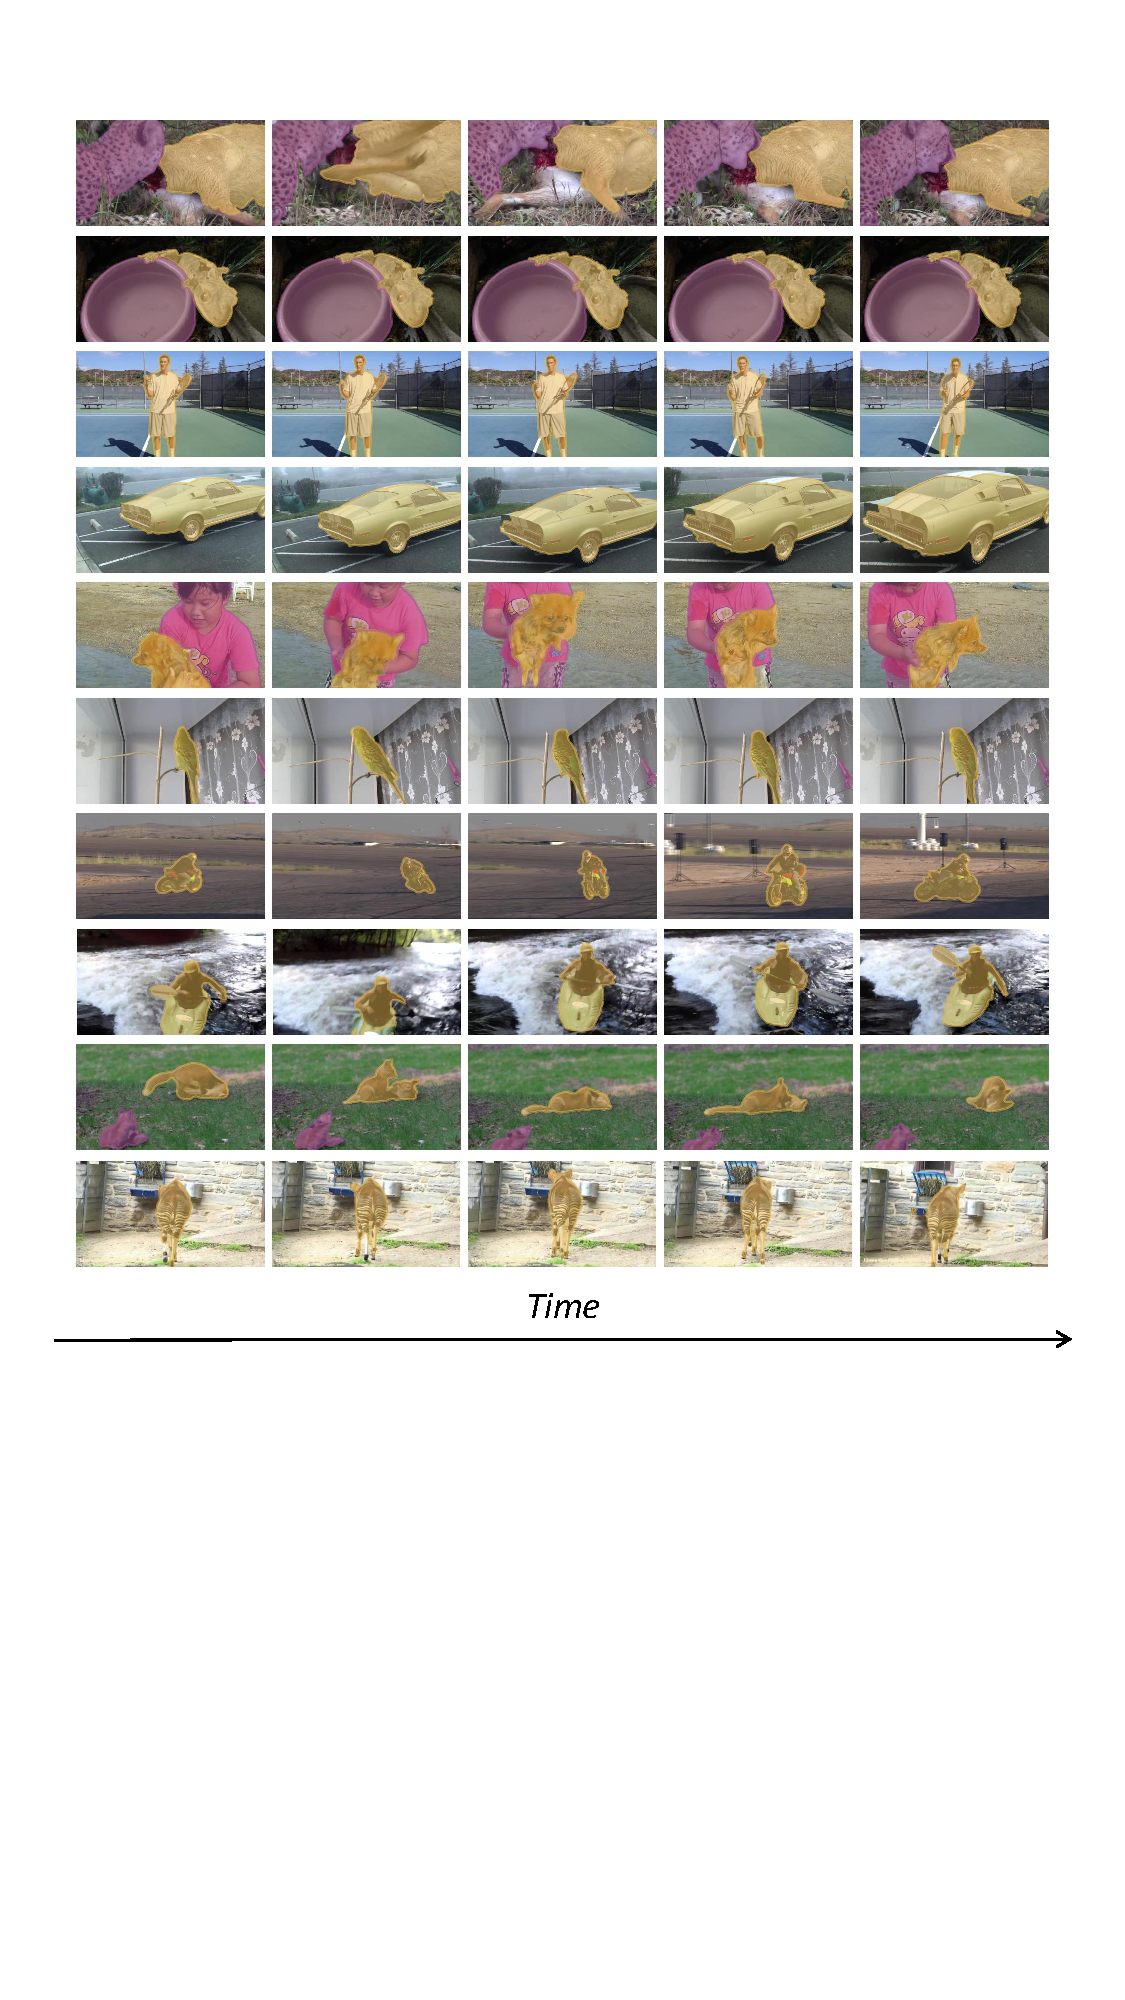
\includegraphics[width=1\linewidth]{figures/sub_vis_figures.pdf}
    \caption{\textbf{Qualitative results of our VIS model on YouTubeVIS-2019 \texttt{val} split.}}
    \label{fig:add_vis_visual}
\end{figure*}

\begin{figure*}[h]
    \centering
    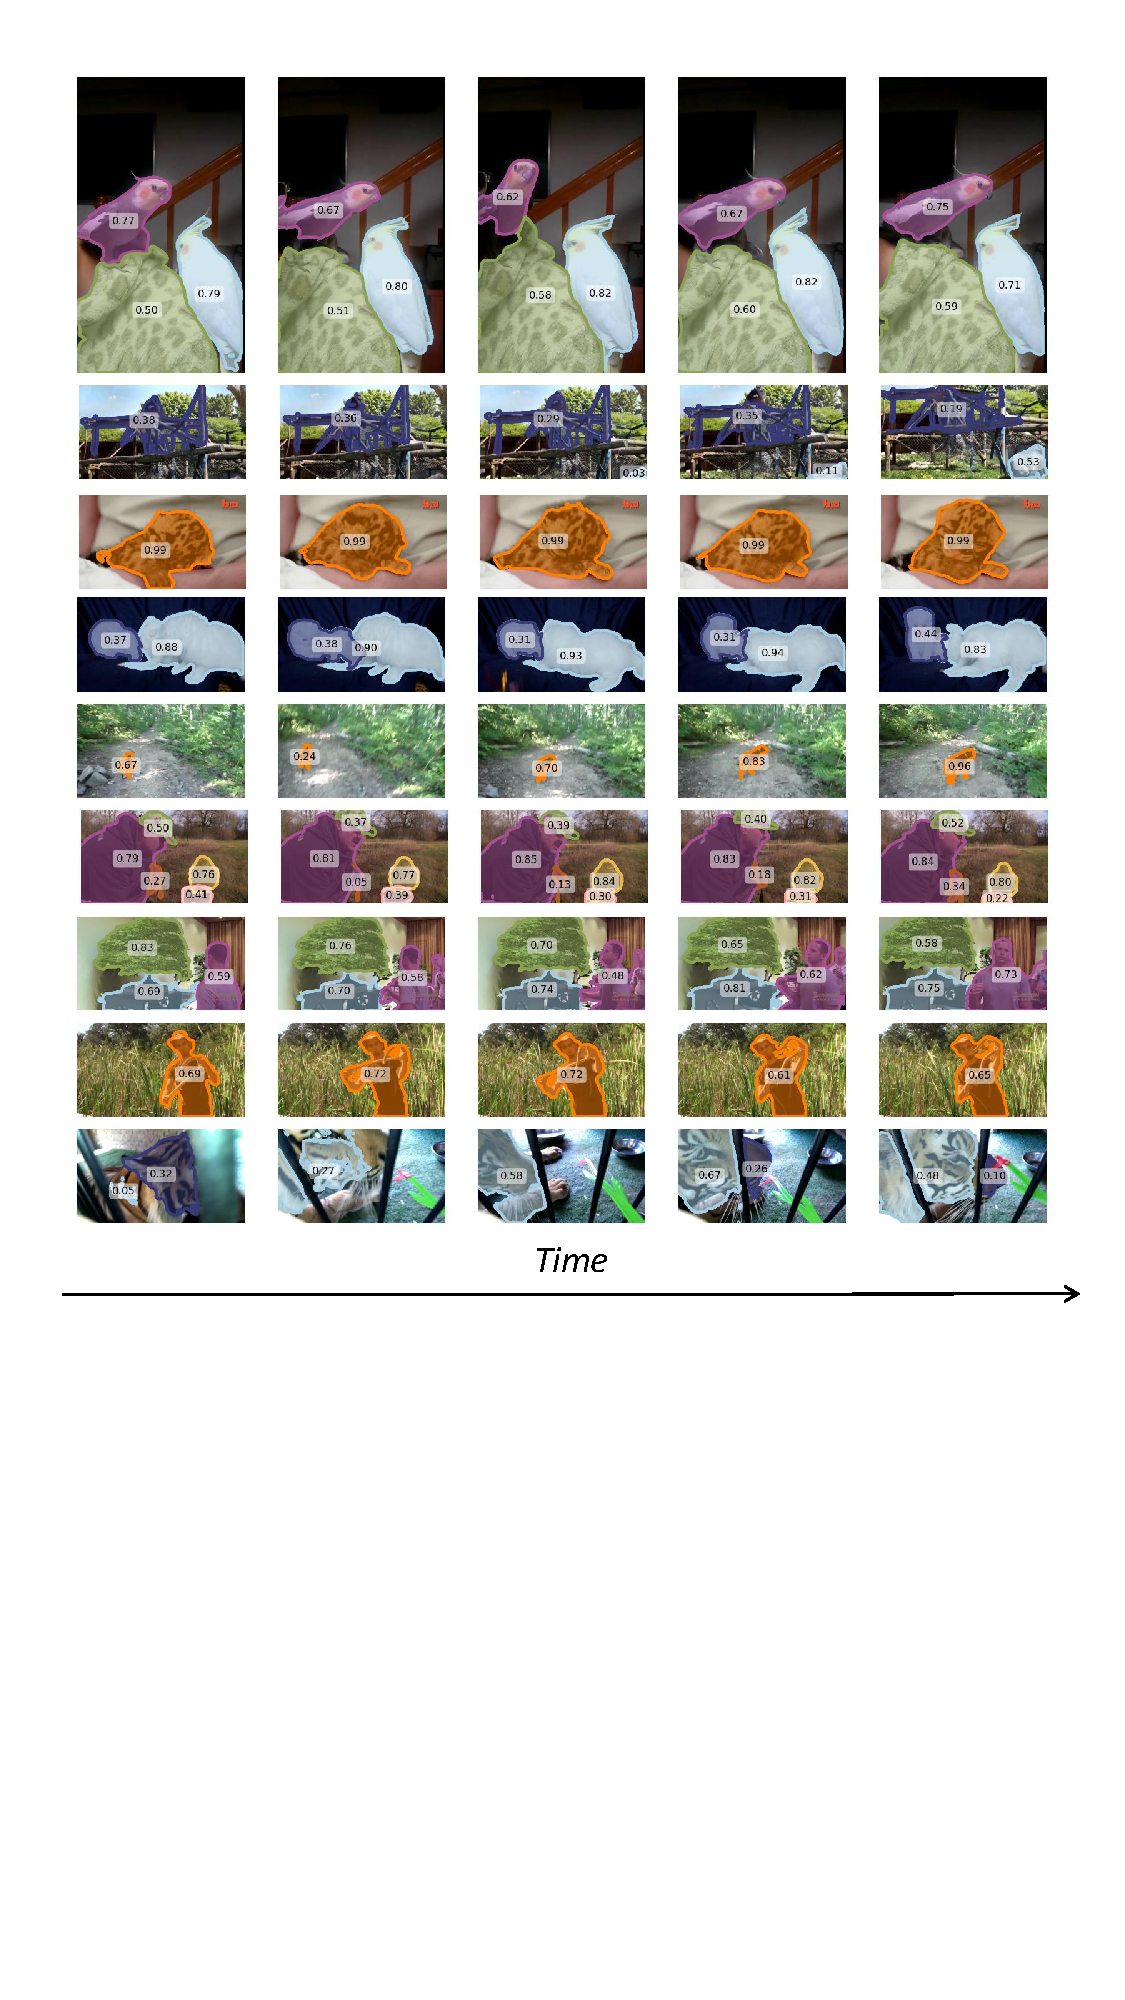
\includegraphics[width=1\linewidth]{figures/sub_quality_figures.pdf}
    \caption{\textbf{Qualitative results of our quality predictor on YouTubeVIS-2019 \texttt{train} split.} The quality scores are shown in the center of each pseudo label.}
    \label{fig:quality_visual}
\end{figure*}

We provide additional qualitative results of our VIS model and quality predictor in \cref{fig:add_vis_visual} and \cref{fig:quality_visual}.